\documentclass{article}
\usepackage{cite}
\usepackage{graphicx} % Required for inserting images
\usepackage{float}

\title{Homework 3: Explanation and causality, scientific laws and regularities}
\author{Casper Kristiansson}
\date{\today}

\begin{document}

\maketitle

\section{Two Research Studies}
\subsection{Study One}
Yes and no. The observed outcome is that group A wrote better programs due to commenting doesn't in every scenario true. This is because while we know that this is a common factor from group A there might be a lot of other factors which may affect the result of the study. For example, group A could have a lot more experience than group B, etc Therefore you cannot draw the concrete conclusion that comments improve code. But even so, if the study had been tested over and over again and thoroughly tested so that both groups have the same skills and knowledge and the commenting group kept showing better results you could draw that conclusion.

This means that the study can be improved by controlling the other variables like skills and knowledge. They are not letting students choose which group but random selection will also improve the results.

\subsection{Study Two}
No, from the study it cannot draw the conclusion that functional programming languages give slower code. The execution time of the solution to the problem that was produced by the different students has a lot of other factors. One of these factors is previous knowledge and skills. For example, we already know that Java is a much more known programming language which would result in students with more experience with it being able to create more optimized and better programs in terms of execution time.

Ways to improve the study would be by controlling so that the amount of experience the students have both with Java and Haskell are similar or equal.

\section{Zipf's Law}

For this exercise, I chose to use the data set Billionaires CORGIS Dataset Project \cite{corgiseduCORGISDatasets}. The dataset contains different parameters of the world's richest billionaires. The parameter that I focused on was the sector parameter. To solve the task I first downloaded the data and inspected it. I then simply ranked and grouped the data and plotted it in using matplotlib. Then using a library like sklearn we can easily perform linear regression on the data. With the given data we can see that it applies to Zipf's law.

Zipf's law can be viewed as a hypothesis because it makes predictions based on a specific relationship like the frequency and ranks of words. What has been seen with Zipf's law is that it has been correct in many different scenarios and areas. But Zipf's law can also be seen as a scientific theory because it has over and over been correct and followed its guidelines.

\begin{figure}[H]
    \centering
    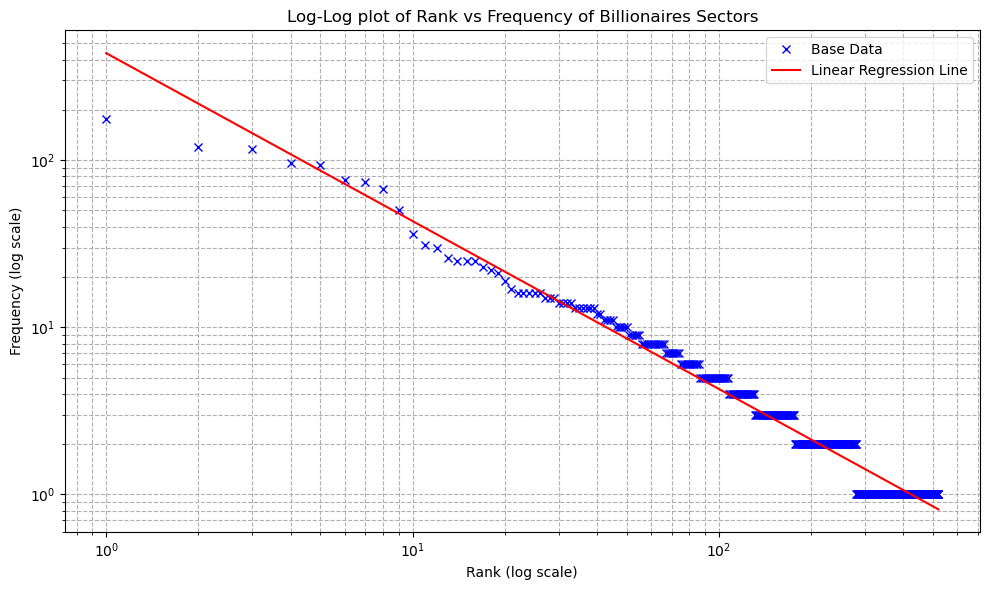
\includegraphics[width=\textwidth]{Graph.png}
    \caption{Log-log plot of rank vs. frequency of Billionaires sectors}
    \label{fig:graph}
\end{figure}

\begin{table}[H]
\centering
\begin{tabular}{|l|c|}
\hline
\textbf{Parameter} & \textbf{Value} \\
\hline
Slope ($-\alpha$) & -1.0047 \\
Intercept ($\log(C)$) & 6.0792 \\
Mean Squared Error& 0.0290 \\
\hline
\end{tabular}
\caption{Linear Regression Fit Variables}
\label{table:linear_regression_details}
\end{table}

\bibliographystyle{IEEEtran}
\bibliography{main}

\end{document}
